% !TEX TS-program = pdfLaTeX
\documentclass[10pt,aspectratio=43,compress,xcolor=x11names,UTF8]{beamer}
\usepackage{xcolor-material}
\usetheme{Darmstadt}
\usecolortheme{seahorse}
\graphicspath{{figure/}} % 图片路径
\usepackage{calligra} % Thank you
\usepackage{ctex} 
\usepackage{natbib} % 参考文献

\title[Spatial Generalized Linear Mixed Models]{Spatial Generalized Linear Mixed Models with Application to Prevalence Mapping}
\subtitle{空间广义线性混合模型及其在预测流行病中的应用\\ 2015级硕士学位论文答辩}
\author[黄湘云 \and 李再兴]{学生:黄湘云 \and 导师:李再兴}

\institute[中国矿业大学(北京)] 
{
  % \inst{1}%
  专业:统计学\quad 方向:数据分析与统计计算 %\\
  % 理学院\quad 中国矿业大学(北京)
}

\date[\today] % (optional)
{
\includegraphics[width=38ex,interpolate=true]{cumtb} \\ ~~\\
\today / 逸夫楼}

\begin{document}

\maketitle

\begin{frame}{Outline}
\tableofcontents
\end{frame}

\section{引言}

\subsection{研究意义}

\begin{frame}{}
\emph{例}\textit{例} \texttt{例} \textsf{例} \textbf{例}
\begin{enumerate}
\item radionuclide concentrations on Rongelap Island
\item childhood malaria in the gambia
\item Loa loa prevalence in Cameroon and surrounding areas
\end{enumerate}

\end{frame}

\begin{frame}{Introduction}
\citet{Diggle2002}
\begin{itemize}
\item First item in the list
\item Second item
\item and so on
\begin{itemize}
\item First item in the list
\item Second item
\item and so on
\end{itemize}
\end{itemize}

\begin{itemize}
\item the effects of child level covariates (age and bed net use)
\item village level covariates (the primary health care and greenness of surrounding vegetation)
\item separate components for residual spatial
\item non-spatial extrabinomial variation
\end{itemize}
$\mathbb{R}^{n}$
$$ \mathsf{\log} \{p_{ij}/(1-p_{ij})\} =\alpha + \beta'z_{ij} + U_{i} + S(x_{i})$$

\end{frame}

\subsection{文献综述}

\begin{frame}
\begin{figure}
\centering
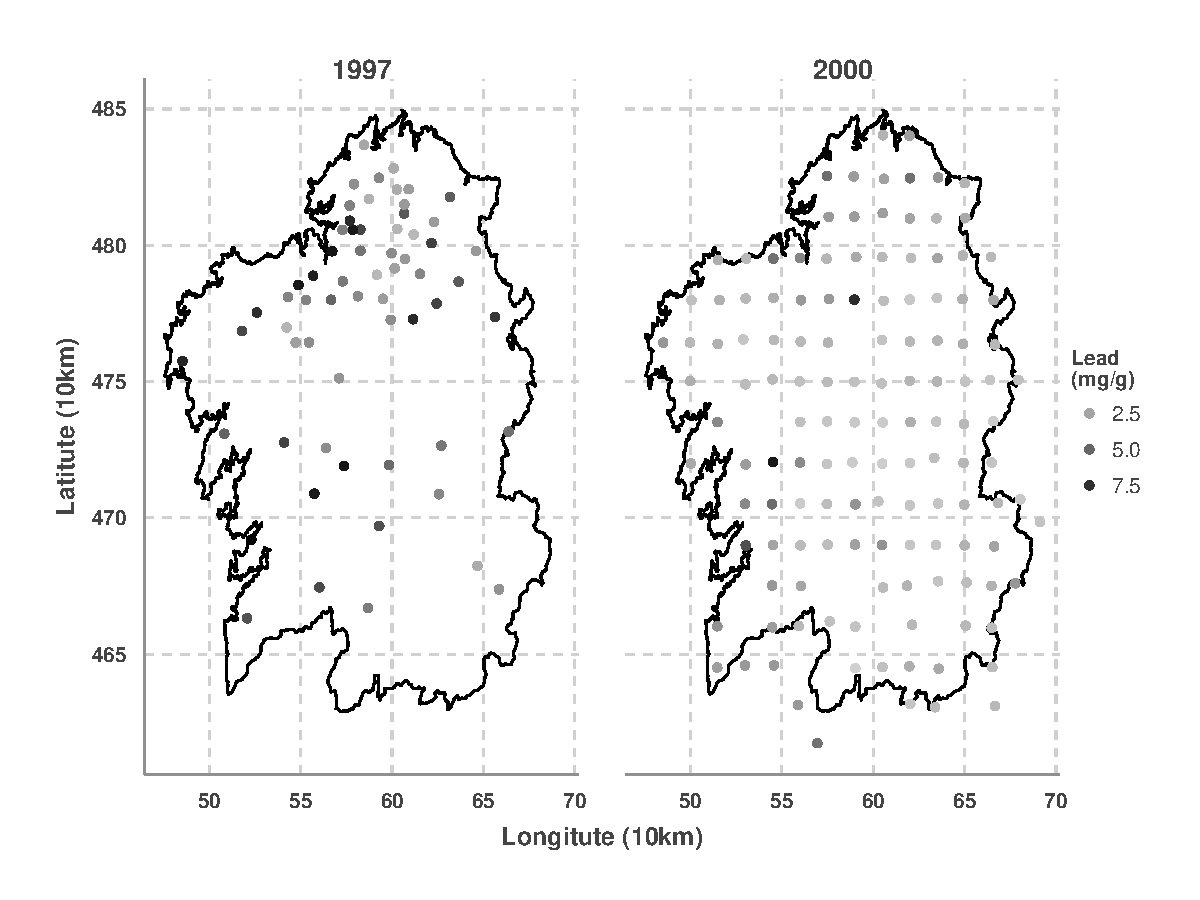
\includegraphics[width=.8\textwidth]{demo04}  
\end{figure}
\end{frame}

\subsection{主要内容}


\section{模型(SGLMM)}

\subsection{模型结构}

\subsection{计算方法}

\subsection{数据分析}

\begin{frame}

The function $f$ is given by
\[ f(x) = 2x + \frac{x - 7}{x^2 + 4}\] 
for all real numbers $x$.

The roots of a quadratic polynomial $a x^2 + bx + c$ with
$a \neq 0$ are given by the formula
\[ \frac{-b \pm \sqrt{b^2 - 4ac}}{2a} \]

The roots of a cubic polynomial of the form $x^3 - 3px - 2q$
are given by the formula
\[ \sqrt[3]{q + \sqrt{ q^2 - p^3 }}
  + \sqrt[3]{q - \sqrt{ q^2 - p^3 }} \]
where the values of the two cube roots must are chosen
so as to ensure that their product is equal to $p$.
\end{frame}

\begin{frame}

{\color{red} \textbf{Multiple prevalence surveys}} \\
Sample $n_{i}$ individuals,observe $Y_{i}$ positives,$i=1,2,\cdots,m$
$$Y_{i}\sim \mathrm{Bin}(n_{i},p_{i})$$

{\color{red} \textbf{Extra-binomial variation}} \\
Sample $n_{i}$ individuals,observe $Y_{i}$ positives,$i=1,2,\cdots,m$
$$Y_{i}|d_{i},U_{i}\sim \mathrm{Bin}(n_{i},p_{i}) \quad 
\log\{p_{i}/(1-p_{i})\}=d_{i}'\beta+U_{i} \quad U_{i} \sim N(0,\tau^2)$$

\textbf{notations:} Spatial Generalized Linear Mixed Models (SGLMM)
\begin{itemize}
\item Latent spatially correlated process \\
Stationary Gaussian Process: $S(x) \sim \mathrm{SGP}\{0,\sigma^2,\rho(u)\} $ \\
correlation function: e.g. $\rho(u)=\exp(-|u|/\phi)$ 
\item Linear prediction (regression model)\\
$d(x)=$ covariates at location $x$\\
Linear prediction: $\eta(x)=d(x)'\beta + S(x)$ \\
Link function: logit $p(x)=\log\{\eta(x)/[1-\eta(x)]\}$ 
\item Conditional distribution for positive proportion $Y_{i}/n_{i}$\\
$Y_{i}|S(\cdot) \sim \mathrm{Bin}(n_{i},p(x_{i}))$ (binomial sampling)
\end{itemize}

\end{frame}

\begin{frame}
Let $\mathbf{u}$,$\mathbf{v}$ and $\mathbf{w}$ be three
vectors in ${\mathbf R}^3$. The volume~$V$ of the
parallelepiped with corners at the points
$\mathbf{0}$, $\mathbf{u}$, $\mathbf{v}$,
$\mathbf{w}$, $\mathbf{u}+\mathbf{v}$,
$\mathbf{u}+\mathbf{w}$, $\mathbf{v}+\mathbf{w}$
and $\mathbf{u}+\mathbf{v}+\mathbf{w}$
is given by the formula
\[ V = (\mathbf{u} \times \mathbf{v}) \cdot \mathbf{w}.\] 

\[ \cos(\theta + \phi) = \cos \theta \cos \phi
      - \sin \theta \sin \phi \]

\[ M^\bot = \{ f \in V' : f(m) = 0 \mbox{ for all } m \in M \}.\] 	  
\end{frame}



\section{结论与展望}

\begin{frame}
\centering {\zihao{0} \color{GoogleRed} \calligra{Thank You}}

\end{frame}



\begin{frame}[allowframebreaks]
\frametitle{参考文献}
\bibliographystyle{authordate1}
\bibliography{R-GLMM-pkgs}
\end{frame}

\appendix

\section*{附录}

\begin{frame}{软件环境}
R 3.4.2
rstan
geoR
geoRglm
INLA
\end{frame}

% OpenBUGS  WinBUGS  JAGS
% library(R2OpenBUGS) # 2017-2-20 version 3.2-3.2
% library(R2WinBUGS) # 2015-07-29 version 2.1-21
% library(rjags) # 2016-02-19 version 4-6
% library(BRugs) # OpenBUGS 2017-06-26  version 0.9-0
% library(glmmBUGS) # Generalised Linear Mixed Models with BUGS and JAGS 2016-09-22 version 2.4.0
% library(R2jags) # Using R to Run 'JAGS'  2015-08-23	 version 0.5-7

% network
	% diagram DiagrammeR DiagrammeRsvg
 % library(help=graph)

 % library(help=Rgraphviz)
 % library(help=igraph)



\end{document} 


